\documentclass[11pt,twocolumn]{article}
\usepackage[letterpaper,top=0.80in,bottom=0.78in,left=0.74in,right=0.74in,columnsep=0.26in]{geometry}
\usepackage[T1]{fontenc}
\usepackage[utf8]{inputenc}
\usepackage{newtxtext,newtxmath}
\usepackage{microtype}
\emergencystretch=1.6em
\usepackage{amsmath,mathtools}
\usepackage{booktabs,array,tabularx,multirow}
\usepackage{graphicx,caption,subcaption}
\usepackage{enumitem}
\usepackage[table]{xcolor}
\usepackage{tikz}
\usetikzlibrary{arrows.meta,positioning,fit,calc,shapes.geometric}
\usepackage[hyphens]{url}
\usepackage[hidelinks]{hyperref}
\usepackage{fancyhdr}
\usepackage{float}
\usepackage{titlesec}
\usepackage{balance}
\usepackage{needspace}
\usepackage{algorithm}
\usepackage{algpseudocode}
\usepackage{listings}
\definecolor{ink}{HTML}{18263A}
\definecolor{royal}{HTML}{3B417B}
\definecolor{pale}{HTML}{F2F4FA}
\definecolor{border}{HTML}{C8D0DF}
\definecolor{muted}{HTML}{5A6878}
\definecolor{teal}{HTML}{0B656E}
\captionsetup{font=footnotesize,labelfont=bf,skip=5pt}
\titleformat{\section}{\large\bfseries\color{ink}}{\thesection}{0.6em}{}
\titleformat{\subsection}{\normalsize\bfseries\color{royal}}{\thesubsection}{0.6em}{}
\titleformat{\subsubsection}{\normalsize\itshape\color{ink}}{\thesubsubsection}{0.5em}{}
\titlespacing*{\section}{0pt}{11pt}{5pt}
\titlespacing*{\subsection}{0pt}{8pt}{3pt}
\titlespacing*{\subsubsection}{0pt}{5pt}{2pt}
\setlength{\parindent}{1em}
\setlength{\parskip}{0pt}
\setlist[itemize]{leftmargin=1.35em,itemsep=1pt,topsep=3pt}
\setlist[enumerate]{leftmargin=1.55em,itemsep=1pt,topsep=3pt}
\newtheorem{definition}{Definition}
\newtheorem{property}{Property}
\newcommand{\mcr}{\textsc{MCR}}
\newcommand{\acla}{\textsc{ACLA}}
\newcommand{\eaf}{\textsc{EAF}}
\newcommand{\sha}{\textsc{SHA-256}}
\newcommand{\evid}{\mathcal{E}}
\newcommand{\auth}{\mathcal{A}}
\newcommand{\mission}{\mathcal{M}}
\newcommand{\caps}{\mathcal{C}}
\newcommand{\obs}{\mathcal{O}}
\newcommand{\action}{\mathcal{X}}
\newcommand{\R}{\mathbb{R}}
\newcommand{\code}[1]{\texttt{#1}}
\newcommand{\smallurl}[1]{\url{#1}}
\hypersetup{pdftitle={From Agent Intent to Verifiable Mission Outcomes: MCR 4.0}, pdfauthor={Prasad Deshpande},pdfsubject={Mission Capability Runtime 4.0 Class A bounded synthetic research}}
\pagestyle{fancy}
\fancyhf{}
\fancyhead[L]{\footnotesize\textcolor{muted}{MCR 4.0 \quad Bounded Synthetic Research Paper}}
\fancyhead[R]{\footnotesize\textcolor{muted}{v1.0.2 Public Review Candidate}}
\fancyfoot[C]{\footnotesize\thepage}
\renewcommand{\headrulewidth}{0.25pt}
\setlength{\headheight}{12pt}
\lstset{basicstyle=\ttfamily\footnotesize,backgroundcolor=\color{pale},breaklines=true,frame=single,rulecolor=\color{border}}
\begin{document}
\twocolumn[{
\begin{center}
{\Large\bfseries\color{ink} From Agent Intent to Verifiable Mission Outcomes:}\\[4pt]
{\Large\bfseries\color{ink} Mission Capability Runtime 4.0}\\[6pt]
{\normalsize\itshape A Versioned, Authority-Bounded Execution and Evidence Architecture for Agentic AI}\\[12pt]
{\normalsize\bfseries Prasad Deshpande}\\[2pt]
{\small Independent Researcher --- Agentic AI Systems and Enterprise Architecture}\\[2pt]
{\small ORCID: 0009-0008-1344-6585 \quad | \quad er.prasad.deshpande@gmail.com}\\[2pt]
{\small \url{https://prasaddeshpande.com} \quad | \quad 26 October 2026}\\[7pt]
{\small \color{muted} Public Review Candidate v1.0.2 \quad $\bullet$ \quad Owner-closed Class A synthetic P1 \quad $\bullet$ \quad Not peer reviewed or production qualified}
\end{center}
\vspace{4pt}
\noindent{\bfseries\color{royal} Abstract}\quad
Autonomous agents can discover tools, propose actions, recover from failure, and generate plausible success narratives. None of these events alone establishes that an enterprise action was authorized, bound to the intended target, executed within constraints, or supported by trustworthy outcome evidence. This paper presents Mission Capability Runtime (MCR) 4.0, a versioned execution-and-evidence architecture that separates model intent from deterministic capability binding, policy authority, bounded retries, observation, and mission disposition. It positions MCR alongside the Agentic Context Lifecycle Architecture (ACLA), which compiles governed mission context, and the Enterprise Agent Framework (EAF), whose research scope includes pre-action authority and independent outcome-assurance responsibilities. The central design rule is \emph{interoperability does not imply authority}. We formalize mission contracts, authorization and revocation gates, execution identities, evidence commitments, and non-promotable uncertainty states. A staged synthetic research program identified material defects in target binding, authorization expiry, nonce and call-budget enforcement, recovery, observer trust, idempotency, and reproducibility; subsequent isolated corrections and fresh Claude Code reviews informed an R6 closure decision. The final executor-supplied R6 receipt reports 131/131 unit tests, 18/18 synthetic scenarios, 22/22 R2 regressions, 40/40 reconciled reviewer tests, 64 adversarial tests, and 45 distinct mutation probes; two original historical reviewer assertions remain failed in the unmodified raw harness (38/40), while the reconciled canonical qualification runner reports 26/26 checks. The owner closed P1 as \code{MCR\_\allowbreak R4\_\allowbreak 0\_\allowbreak P1\_\allowbreak CLOSED\_\allowbreak BOUNDED\_\allowbreak SYNTHETIC\_\allowbreak RESEARCH}. A subsequent owner-local read-only audit reported byte-level verification of the private R6 archive and consistent test receipts; it did not rerun the tests. This manuscript preparation environment did not itself access the private archive. We make no claim of live ACLA/EAF interoperability, SAP authority, production deployment, generalized exactly-once semantics, or verified business outcomes. The contribution is an inspectable systems design, a falsifiable qualification method, and a carefully bounded synthetic finding rather than a production certification.
\vspace{6pt}
\noindent{\bfseries Keywords:} agentic AI; execution assurance; capability binding; authorization; revocation; idempotency; evidence integrity; provenance; synthetic qualification; independent review; enterprise agents
\vspace{10pt}
}]

\section{Introduction}
Enterprise agents are increasingly described in terms of their ability to reason, select tools, coordinate workflows, and recover from errors. Such descriptions conceal a critical boundary: an agent may be able to \emph{propose} an action without being authorized to \emph{perform} it, and it may observe a successful tool response without possessing credible evidence that the intended business state changed. The distinction is especially consequential where the tools represent mutable systems of record, asynchronous processes, or policy-controlled environments. Failure modes are not confined to model hallucination. They arise from stale authorization, mismatched target identities, replayed requests, ambiguous timeout outcomes, insecure retry behavior, observer failures, and unsupported assertions of completion.

The Mission Capability Runtime (MCR) research program examines this boundary. Earlier MCR versions progressed from bounded mission control and offline evidence toward a closed MCR 3.0 reference. MCR 4.0 selects a distinct architecture: \emph{Option B}, a versioned evidence and execution-assurance runtime with independently owned adapters. Its responsibility is neither to persist all model knowledge nor to replace enterprise policy engines. Instead, MCR mediates a defined transition from validated mission intent to controlled execution and evidence-backed disposition. It must refuse to infer missing authority or elevate uncertain outcomes into success.

This research is presented as a member of a broader architectural family. ACLA separates large historical knowledge from governed, mission-bounded context and provenance \cite{deshpandeACLA}. EAF is an adjacent research program concerned with authority, policy, pre-action assurance, and independent outcome assurance \cite{deshpandeEAF}; its exact implemented integration with MCR 4.0 is not established by the present evidence. MCR adds capability binding, orchestration state, retry and recovery discipline, evidence preservation, and a final mission decision. Engineering telemetry and owner-facing approval interfaces remain downstream, non-authoritative consumers unless authority is independently established.

\subsection{Research question and hypotheses}
The principal research question is:
\begin{quote}\small\emph{Can a deterministic, authority-bounded mission runtime preserve execution identity, reject unsafe transitions, and retain reproducible evidence across synthetic adversarial scenarios without treating model, tool, or telemetry claims as proof of authorization or outcome?}\end{quote}
We analyze three hypotheses:
\begin{itemize}
\item \textbf{H1 (authority safety):} binding an approved mission to explicit target, capability, validity, and call constraints can cause unauthorized synthetic transitions to fail closed.
\item \textbf{H2 (outcome integrity):} execution evidence, independent observation, and explicit UNKNOWN disposition can distinguish attempted action from verified outcome within the declared test model.
\item \textbf{H3 (review-driven hardening):} adversarial independent model-session reviews and mutation probes can reveal material defects omitted by an initial passing synthetic harness.
\end{itemize}
The corresponding falsification events include a forbidden call being accepted, a stale or mismatched authority being reused, a tampered evidence field surviving canonical qualification, a repeated mutation producing a duplicate unintended effect, or an UNKNOWN execution being marked as a newly authorized success without validation. These hypotheses address a \emph{synthetic test universe}; universal enterprise claims require new experiments.

\subsection{Contributions and claim boundary}
This paper contributes: (1) a clean five-role separation among context, assurance, execution, observability, and owner interaction; (2) a formal, testable model of capability binding and mission disposition; (3) a contract-first Class A boundary with immutable schema digests; (4) an adversarial qualification history that preserves negative results; (5) a reproducibility and claim-to-evidence protocol; and (6) a bounded interpretation of the R6 closure. The work does \emph{not} claim to invent authorization, state machines, transactional execution, provenance, or mutation testing. Its novelty claim is the particular integration of these concerns into an inspectable agent-runtime research program under deliberately narrow empirical support.

\section{Problem Definition and Boundaries}
\subsection{Intent is not executable authority}
A language model can emit a mission proposal $q$, a candidate tool $c$, and arguments $a$. Yet the executable decision depends on more than those outputs. We distinguish the model's descriptive proposal $P$ from a gate-controlled, versioned execution envelope $V$ and a separately validated authorization state $A_t$:
\begin{equation}
P=(q,c,a) \quad\not\Rightarrow\quad \mathrm{AllowExecute}(P,t).
\label{eq:intent}
\end{equation}
Let $B(q,c,e)$ be a deterministic binding predicate that relates mission $q$, capability $c$, and approved envelope $e$. Let $\mathrm{ValidAuth}(e,t)$ test the currently observed authorization, including expiry and revocation checks required by the contract. A minimal admissibility specification is:
\begin{equation}
\begin{split}
\mathrm{AllowExecute} =\;& B(q,c,e) \wedge \mathrm{ValidAuth}(e,t)\\
&\wedge\mathrm{BudgetOK}(e)\wedge\mathrm{NonceFresh}(e).
\end{split}
\label{eq:admissibility}
\end{equation}
Equation~\ref{eq:admissibility} is a \emph{research abstraction}, not a verbatim transcription of schema fields or executable source. Its purpose is to make safety predicates explicit and falsifiable.

\subsection{Completion requires an observation contract}
Let $X$ be an execution attempt, $T$ a tool-level acknowledgement, and $O$ a separately evaluated outcome observation. The distinctions are:
\begin{equation}
X \neq T \neq O \neq \mathrm{VerifiedBusinessOutcome}.
\label{eq:states}
\end{equation}
A tool response may establish a transport result but cannot alone assert durable application state. An observer may see an output without sufficient provenance or authority to speak for the target. A deterministic runtime must preserve each layer as a separate evidence class and make missing or contradictory support visible.

\subsection{Research scope}
The qualified MCR 4.0 result is restricted to \textbf{Class A bounded synthetic research}. The approved contracts are frozen, and synthetic adapters exercise structured workflows under constructed adverse conditions. Class B adapters, real ACLA/EAF/Claude Mods/Prasad Twin interoperability, SAP reads/writes, enterprise credential flow, production-grade operational controls, and live end-to-end business outcomes are outside the decision. Earlier MCR 2.0 and 3.0 findings form background lineage only; they are not silently counted as MCR 4.0 enterprise evidence.

\begin{table}[t]
\centering\caption{Authority and evidence distinctions in the proposed runtime.}
\label{tab:distinctions}
\footnotesize
\begin{tabularx}{\columnwidth}{@{}p{0.32\columnwidth}X@{}}
\toprule
\textbf{Not equivalent} & \textbf{Required distinction}\\\midrule
Tool visible $\neq$ tool permitted & Discovery yields candidates, not authorization.\\
Approval ref. $\neq$ authority & Verify issuer, scope, expiry, revocation and binding.\\
Retry $\neq$ safe replay & Unknown commit state needs explicit recovery.\\
Response $\neq$ outcome & External observation and contract predicates remain required.\\
Hash $\neq$ trust & Integrity does not establish truthful source or identity.\\
Reviewer PASS $\neq$ peer review & Fresh model execution is not human scientific review.\\
Synthetic PASS $\neq$ production & Environment, failures and authorities differ.\\\bottomrule
\end{tabularx}
\end{table}

\section{Related Work and Positioning}
\subsection{Agent context and assurance}
ACLA explores authority-aware selection and compilation of a mission working set, keeping historical knowledge separate from active inference content \cite{deshpandeACLA}. The MCR question is complementary: once a sufficiently governed mission description exists, what mechanism restricts tool invocations and produces evidence-backed disposition? This is not equivalent to compressing context, and MCR does not claim ACLA's experimental token reductions as its own. EAF supplies a conceptual assurance boundary; the present P1 only freezes interoperability contracts for synthetic exercise. The three may be composed architecturally, but there is no verified live integrated experiment in this record.

\subsection{Security governance and authority}
NIST's AI RMF and its Generative AI Profile provide risk-governance lenses, while NIST SP 800-53 distinguishes access control, identification, audit, and assessment families \cite{nistAirmf,nistGai,nist80053}. OWASP's guidance on excessive agency emphasizes minimizing tool functionality, permissions, and autonomy, as well as complete mediation and human approval for consequential actions \cite{owaspAgency}. The MCR architecture operationalizes analogous principles as versioned predicates and negative tests, but it is not assessed or certified against those frameworks.

\subsection{Distributed execution and provenance}
Distributed systems research reminds us that event order, concurrency and partial knowledge require explicit modeling \cite{lamport1978}. Content hashes and canonical serializations can make bytes comparable, but only under fixed encoding and trust assumptions. RFC 8785 specifies a JSON canonicalization method relevant to consistent hashing \cite{rfc8785}; the frozen MCR schema digests do not by themselves prove use of that specific RFC. Software-supply-chain frameworks such as in-toto and SLSA demonstrate the value of independently checked provenance and attestation chains \cite{intoto2019,slsa11}. MCR's evidence discipline is conceptually related, but the submitted P1 record does not assert conformance to in-toto or any SLSA level.

\subsection{Mutation testing as a research instrument}
Mutation testing assesses whether tests detect deliberately perturbed behavior, while equivalent or redundant mutants complicate interpretation \cite{jia2011}. That distinction matters for R6: its receipt reports 45 distinct mutants, 39 raw detections, four material survivors subsequently killed by supplementary probes, and two bounded redundancies retained. The result is not simply an undifferentiated 45/45 raw mutation pass.

\section{MCR 4.0 Architectural Model}
\subsection{Option B: versioned runtime and independent adapters}
Figure~\ref{fig:architecture} depicts the selected five-role organization. The evidence contract is deliberately stronger than a shared schema: it defines distinct sources of claims, the authority responsible for each decision, and the conditions under which a status can be promoted. In particular, telemetry and owner-facing screens must not acquire implicit execution authority.

\begin{figure*}[t]
\centering
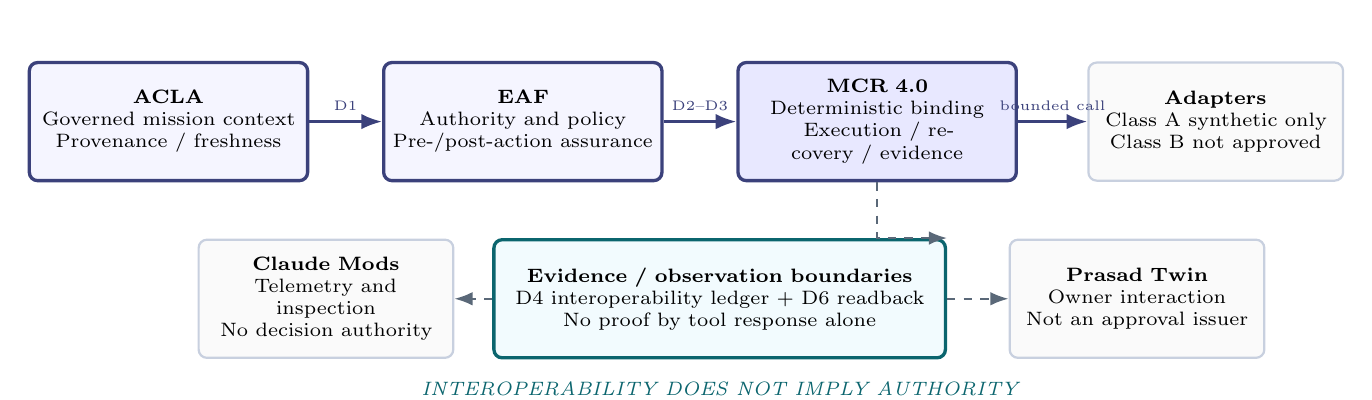
\begin{tikzpicture}[>=Latex, font=\scriptsize,
 unit/.style={draw=royal,very thick,rounded corners=3pt,align=center,minimum height=15mm,text width=33mm,fill=blue!4},
 contract/.style={draw=teal,very thick,rounded corners=3pt,align=center,minimum height=15mm,text width=55mm,fill=cyan!5},
 side/.style={draw=border,thick,rounded corners=3pt,align=center,minimum height=15mm,text width=30mm,fill=gray!4},
 arr/.style={->,line width=1pt,color=royal}]
\node[unit] (acla) at (0,0) {\textbf{ACLA}\\Governed mission context\\Provenance / freshness};
\node[unit] (eaf) at (4.5,0) {\textbf{EAF}\\Authority and policy\\Pre-/post-action assurance};
\node[unit,fill=blue!9] (mcr) at (9,0) {\textbf{MCR 4.0}\\Deterministic binding\\Execution / recovery / evidence};
\node[side] (adapter) at (13.3,0) {\textbf{Adapters}\\Class A synthetic only\\Class B not approved};
\draw[arr] (acla) -- node[above,font=\tiny]{D1} (eaf);
\draw[arr] (eaf) -- node[above,font=\tiny]{D2--D3} (mcr);
\draw[arr] (mcr) -- node[above,font=\tiny]{bounded call} (adapter);
\node[contract] (evidence) at (7,-2.25) {\textbf{Evidence / observation boundaries}\\D4 interoperability ledger + D6 readback\\No proof by tool response alone};
\node[side] (mods) at (2,-2.25) {\textbf{Claude Mods}\\Telemetry and inspection\\No decision authority};
\node[side] (twin) at (12.3,-2.25) {\textbf{Prasad Twin}\\Owner interaction\\Not an approval issuer};
\draw[->,dashed,thick,color=muted] (mcr.south) |- (evidence.north east);
\draw[->,dashed,thick,color=muted] (evidence.west) -- (mods.east);
\draw[->,dashed,thick,color=muted] (evidence.east) -- (twin.west);
\node[font=\scriptsize\itshape,color=teal] at (7,-3.4) {INTEROPERABILITY DOES NOT IMPLY AUTHORITY};
\end{tikzpicture}
\caption{The selected MCR 4.0 \emph{Option B} architecture. Arrows depict contract roles and an intended integration topology, not verified live interoperation. The Class A synthetic runtime exercises the boundary without granting external authority.}
\label{fig:architecture}
\end{figure*}

\subsection{Five independent responsibility planes}
\textbf{Context plane (ACLA).} Compiles task-sufficient, authority-aware context and distinguishes active working sets from long-lived provenance. The D1 contract represents compiled context, but context validity is not an execution permit. \textbf{Assurance plane (EAF).} Owns pre-action authority/policy control and independent outcome assurance, modeled through D2 and D3 boundaries. \textbf{Mission execution plane (MCR).} Binds approved capability to the intended identity, bounds calls, manages retry and recovery, commits evidence, and renders a mission disposition. \textbf{Observability plane (Claude Mods).} Presents telemetry and engineering traces without authority to rewrite decisions. \textbf{Owner interaction plane (Prasad Twin).} Presents decisions and approval requests; the interface is not itself a substitute approval signer or a second Twin Brain. These are \emph{architectural allocations}, not claims of finished interoperation.

\subsection{The Class A interoperability contracts}
Six versioned schema artifacts constitute the frozen Class A baseline (Table~\ref{tab:contracts}). Owner approval is captured as user-message provenance and associated exact SHA-256 values, not as an independent cryptographic identity attestation. A schema digest controls identity of bytes; it does not establish that the schema can safely govern a live enterprise. Any Class B extension requires a new authorization decision rather than silent promotion.

\begin{table*}[t]
\centering\caption{Owner-frozen Class A contract identities, baseline v1.0.0. Exact digests are recorded from the research handover and closure record; not rehashed in this authoring environment.}
\label{tab:contracts}
\small
\begin{tabularx}{\textwidth}{@{}p{0.045\textwidth}p{0.31\textwidth}X@{}}
\toprule
\textbf{ID} & \textbf{Contract role} & \textbf{SHA-256 digest}\\\midrule
D1 & ACLA compiled context & \texttt{d91d441b9363\allowbreak 1c9c645399a5\allowbreak 37c96041e023\allowbreak f406f93571a8\allowbreak f9b0a0704817\allowbreak 0a62}\\
D2 & EAF MissionExecutionEnvelope & \texttt{19839a19b97c\allowbreak 1e665d1b322e\allowbreak 4f45668b292e\allowbreak 9e943b121641\allowbreak 372592cf7a1d\allowbreak e724}\\
D3 & Authorization and revocation & \texttt{530943d21988\allowbreak d02527504115\allowbreak fc500b90b759\allowbreak feea25aeeef9\allowbreak ebec347e0d05\allowbreak ad07}\\
D4 & MCR evidence interoperability & \texttt{02e694493a4c\allowbreak 3fc7b74aa3eb\allowbreak b2d6d46beb5f\allowbreak 15d7bcc16348\allowbreak d722b3997e35\allowbreak c554}\\
D5 & Prasad Twin approval interface & \texttt{60c553bf62f2\allowbreak 8c40653f7b27\allowbreak 0f4894f2b237\allowbreak 6d3219c8d4da\allowbreak c4415c7be3ae\allowbreak e6bc}\\
D6 & Outcome observation and readback & \texttt{876b45505e1a\allowbreak 3daa762b5485\allowbreak 85a50d73cc73\allowbreak 6960553a8ea4\allowbreak 26c5e0805865\allowbreak ba0b}\\\bottomrule
\end{tabularx}
\end{table*}

\section{Formal Execution and Evidence Model}
\subsection{Mission and capability identity}
\begin{definition}[Mission instance]
A mission is a tuple $m=(\mathrm{id},q,v,\sigma,r)$ where $\mathrm{id}$ is its stable identity, $q$ its requested objective, $v$ its declared contract version, $\sigma$ its constraints and $r$ its required outcome predicates. This notation is an analytical model; deployed field names must be read from the actual frozen schemas.
\end{definition}
\begin{definition}[Qualified capability]
A candidate capability $c$ is qualified for a mission only if an explicit binding $\beta(m,c,t)$ evaluates true for the intended target and approved scope at decision time $t$. Discovery, tool metadata, or model confidence alone cannot satisfy $\beta$.
\end{definition}
Thus:
\begin{equation}
Q(c,m,t)=\mathbb{1}[\beta(m,c,t)]\;\mathbb{1}[\mathrm{Auth}(m,c,t)].
\label{eq:qual}
\end{equation}
A useful target-binding invariant is:
\begin{equation}
\forall x:\ \mathrm{Exec}(x)\Rightarrow
\mathrm{Target}(x)=\mathrm{ApprovedTarget}(m).
\label{eq:target}
\end{equation}
The two predicates are necessary for admissibility in this model, but do not alone guarantee safe execution. Capability quality, time-of-check/time-of-use races and external system behavior remain additional concerns.

\subsection{Authorization freshness and revocation}
Authority should be checked at every protected transition, especially at resume from ambiguous state. Let $t_e$ denote authority expiry and $R_t$ denote revocation state:
\begin{equation}
\mathrm{Auth}(t)=\mathrm{IssuerOK}\land (t<t_e)\land\neg R_t\land\mathrm{ScopeOK}.
\label{eq:revocation}
\end{equation}
An invalid or incomparable timestamp must not be converted into permission. F1 in the historical review concerned invalid or incorrectly compared expiry timestamps; F3 concerned an UNKNOWN recovery path presenting prior ALLOW as current authorization. The model therefore requires a fresh check rather than a cached boolean carried across resumed execution.

\subsection{Call budget, nonce and replay safety}
For envelope $e$, define $k_e$ as calls already committed to its accounting scope and $K_e$ as its maximum permitted calls. Then
\begin{equation}
\mathrm{BudgetOK}(e)\iff k_e<K_e.
\label{eq:budget}
\end{equation}
Nonces, envelope digests and idempotency identities prevent a correctly shaped request from being reused in a different mission context without explicit verification. The exact replay guarantees depend on durable adapter semantics. An idempotency key cannot retroactively guarantee that a remote side effect occurred only once if the external system does not support suitable semantics.

\subsection{Unknown outcomes and recovery}
The runtime needs at least a three-valued mission outcome vocabulary, even when the test harness implements more detailed state distinctions:
\begin{equation}
D(m)\in\{\mathrm{SUCCESS},\mathrm{FAILURE},\mathrm{UNKNOWN}\}.
\label{eq:outcome}
\end{equation}
The safe rule is:
\begin{equation}
D(m)=\mathrm{SUCCESS}\Rightarrow
\bigwedge_{p\in r}\mathrm{Supported}(p,\evid_{m}).
\label{eq:success}
\end{equation}
If observation is unavailable, stale, source-ambiguous, or compromised, the disposition must not be promoted to SUCCESS. Recovery from UNKNOWN is a new decision point requiring authorization and observation reconciliation, not just a replay of the previous ALLOW flag.

\begin{figure}[t]
\centering
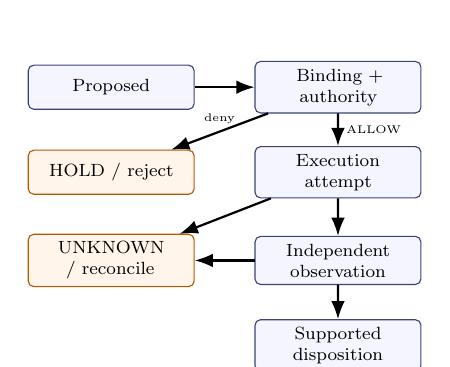
\begin{tikzpicture}[>=Latex,scale=0.8,transform shape,
 node/.style={draw=royal,rounded corners=2pt,fill=blue!4,text width=24mm,align=center,minimum height=7mm,font=\footnotesize},
 warn/.style={draw=orange!70!black,rounded corners=2pt,fill=orange!8,text width=24mm,align=center,minimum height=7mm,font=\footnotesize},
 arr/.style={->,thick}]
\node[node] (propose) at (0,0) {Proposed};
\node[node] (validate) at (3.6,0) {Binding + authority};
\node[node] (attempt) at (3.6,-1.35) {Execution attempt};
\node[warn] (unknown) at (0,-2.75) {UNKNOWN / reconcile};
\node[node] (observe) at (3.6,-2.75) {Independent observation};
\node[node] (final) at (3.6,-4.10) {Supported disposition};
\node[warn] (stop) at (0,-1.35) {HOLD / reject};
\draw[arr] (propose) -- (validate);
\draw[arr] (validate) -- node[right,font=\tiny]{ALLOW} (attempt);
\draw[arr] (validate) -- node[above,font=\tiny]{deny} (stop);
\draw[arr] (attempt) -- (observe);
\draw[arr] (attempt) -- (unknown);
\draw[arr] (observe) -- (final);
\draw[arr] (observe.west) -- ++(-0.35,0) |- (unknown.east);
\end{tikzpicture}
\caption{Research abstraction of the guarded execution transition. UNKNOWN cannot become ALLOW without revalidation. This is not a verbatim implementation state diagram.}
\label{fig:state}
\end{figure}

\subsection{Evidence commitments and independent observation}
Let $E_i$ be a typed event and $d_i$ a digest of its canonicalized commitment. For an append-only evidence sequence, a common reference model is:
\begin{equation}
h_i=H(h_{i-1}\Vert\mathrm{encode}(E_i)\Vert d_i).
\label{eq:ledger}
\end{equation}
Hash-linked structures make modification detectable relative to a trusted checkpoint, but do not authenticate the original sensor or make the observation true. R4B findings F4 and F5 concerned insufficient observer provenance/trust and uncommitted scenario counters or observations. The corrected design requires explicit commitments to the fields that underpin reported test outcomes; a reviewer must inspect which exact fields are covered before inferring integrity.

\subsection{Safety properties and liveness}
\textbf{S1 target safety.} No synthetic execution against a target different from the approved target. \textbf{S2 authority continuity.} Authorization is checked at the appropriate transition, including resume. \textbf{S3 replay control.} An admissible attempt does not exceed its call/nonce envelope. \textbf{S4 evidence non-substitution.} Telemetry, a tool acknowledgement, or an approval reference cannot substitute for verified outcome support. \textbf{S5 provenance preservation.} Once a test outcome or observation is committed to the qualification record, post-review silent mutation must be detectable. \textbf{L1 recovery progress.} Local observer exceptions should not permanently wedge an idempotency key when documented recovery conditions are met. These are design requirements supported by reported synthetic probes, not universal formally verified properties.

\section{Adversary, Trust, and Failure Model}
\subsection{Adversarial principals and surfaces}
The synthetic threat model distinguishes a mission author, a model-facing planner, an authorization issuer, an executor, a capability adapter, an outcome observer, and an evidence verifier. This separation is conceptual; P1 did not authenticate a real enterprise principal for each role. The adversary is permitted to supply malformed or conflicting context, stale approvals, altered targets, replayed envelopes, inconsistent timestamps, tampered evidence, misleading tool acknowledgements, and interruption at consequential boundaries. The adversary is not assumed to break standard cryptographic hash functions. Compromise of the underlying operating system, a genuine signing key, or a real enterprise policy issuer is not within the reproduced experiment.

A central concern is \emph{role confusion}: accepting statements from one role as if they had been certified by another. The planner can suggest an action but not grant authorization. The capability adapter can return a tool response but not independently certify the target's durable business state. The observer can produce a reading, yet its provenance and relationship to the relevant target must be checked. The owner-facing Twin can display an approval request, but it cannot turn an interface click or reference string into issuer-validated authority unless the separate approval system actually confirms it. The same boundary holds for signed manifests: integrity of bytes does not establish the correctness of the embedded conclusions.

\subsection{Failure model for ambiguous execution}
A state-changing remote call can fail in several observably similar ways. A transport timeout may occur before the target receives a request, after it receives the request but before it commits, after it commits but before it responds, or after an observer sees an earlier version of state. Without an authoritative idempotency contract or an independent target-side read, these conditions are not distinguishable merely from the timeout itself. The research runtime must therefore represent uncertainty rather than infer success or blindly retry. The R6 synthetic outcome addresses recovery branches; no evidence is supplied that every possible enterprise ambiguous-commit state has been exhausted.

A qualified retry is not simply a second attempt. It requires at minimum a renewed authority decision, the same approved target identity, a bounded attempt budget, a trustworthy replay identity, and a strategy for distinguishing duplicate effects. If a remote system provides no safe replay or readback primitive, the justified disposition may remain UNKNOWN pending human or target-authoritative resolution. This fail-closed possibility is an intended property, not a sign that the orchestrator is incomplete.

\subsection{Protected transition ledger}
Table~\ref{tab:attacks} maps the major adversarial concerns to the evidence the reviewer would need. The acceptance evidence in the final column is a requested proof artifact, not a claim that a corresponding production control is deployed.
\begin{table*}[t]
\centering\caption{Threat-to-check mapping used to reason about MCR synthetic coverage. Historical finding IDs are evidence-derived; control intent is a research interpretation.}
\label{tab:attacks}
\footnotesize
\begin{tabularx}{\textwidth}{@{}p{0.14\textwidth}p{0.25\textwidth}p{0.25\textwidth}X@{}}
\toprule
\textbf{Threat} & \textbf{Prohibited promotion} & \textbf{Research mitigation intent} & \textbf{Acceptable proof category}\\\midrule
Target substitution (R2) & Context-selected target becomes approved target & Bind executable call to the approved target identity & Negative synthetic call trace + verified no side effect\\
Expired authority (F1) & Malformed or expired token becomes ALLOW & Strict comparable time / issuer / scope check & Rejection tests at and beyond expiry boundary\\
Envelope replay (F2) & Correct shape bypasses nonce or maxCalls & Digest, nonce and bounded-counter checking & Replay and limit-crossing adversarial cases\\
UNKNOWN resume (F3) & Prior ALLOW treated as current authority & Revalidate on recovery decision & Stale/revoked resume negative probes\\
Observer substitution (F4) & Untrusted sensor confirms business state & Typed source and provenance gates & Independent observation-source checks\\
Evidence rewrite (F5) & Altered counters remain apparently valid & Commit result-affecting fields to integrity chain & Hash/manifest corruption negative controls\\
Idempotency wedge (F6) & Observer crash strands later safe progress & Recoverable, bounded lease/state handling & Crash-injection regression and final disposition\\
Missing proof object (F7) & Reported Git SHA treated as local proof & Verify exact commit object and tree & Isolated repository object readback\\
Generated drift (F8) & Incidental artifacts contaminate proof set & Ignore/clean deterministically under rules & Manifest and tracked/untracked state comparison\\\bottomrule
\end{tabularx}
\end{table*}

\subsection{Illustrative counterexamples}
Consider a synthetic mission approved for target $A$ while the model proposes a tool URI for target $B$. A correct control decision is reject, even if the URI is syntactically valid and the model describes $B$ as equivalent. Next consider a mission that previously received ALLOW but resumes from UNKNOWN after an authority revocation. A correct control decision is a fresh denial or deferred resolution, not recovery under the earlier ALLOW. Finally, consider a successful tool acknowledgement followed by a failed or provenance-invalid readback. The only defensible disposition is bounded uncertainty or failure under the declared policy, not a verified success. These examples illustrate required predicates; they are not quoted transcripts from the private R6 packet.

\section{Design Alternatives and Version Lineage}
\subsection{Why the selected architecture is separate}
An alternative would embed all orchestration state and validation into a conversational model's context. That approach would allow a model to reason about retries but would entangle mutable prompt state with authority decisions and weaken reproducibility. Another alternative would use a single central runtime to own context, authorization, execution, review, and user interaction. Such a monolith might simplify a diagram but would amplify the consequences of one compromised component and blur organizational ownership. Option B instead uses independently owned adapters and versioned contracts, requiring explicit translation and validation at each boundary. This is an architectural selection documented in the owner handover, not a comparative benchmark proving Option B superior.

A further alternative is to rely on tool-native guarantees alone. Where tools provide strong idempotency, atomic transaction semantics, authenticated readback and scoped authorization, those controls should be reused rather than duplicated. Yet the orchestrator still needs a deterministic way to bind the mission to those capabilities, represent gaps, and refuse to promise stronger guarantees than the tool supplies. MCR is therefore an assurance-aware coordinator, not a replacement for target-specific transaction or policy infrastructure.

\subsection{Version lineage without retroactive promotion}
MCR 1.9 is recorded as historically frozen with bounded unresolved create-commit state. MCR 2.0 retains a bounded live-outcome reference. MCR 3.0 was closed as \code{CLOSED\_\allowbreak OFFLINE\_\allowbreak BOUNDED\_\allowbreak RESEARCH}, with a qualified merged Git reference and a separately recovered proof checkout. The MCR 4.0 decision is not simply ``MCR3 plus new diagrams'': it adopts versioned interoperability contracts across ACLA/EAF/MCR/Twin boundaries and subjects a new Class A synthetic cross-runtime harness to adversarial qualification. Nonetheless, provenance from older stages is lineage evidence, not an automatic performance or live-outcome claim for MCR 4.0.

The exact MCR 3.0 commit matters because an offline verifier cannot reconstruct history from a textual identifier alone. Conversely, even when the commit and tree are verified, the frozen MCR3 result remains bounded. R5A's isolated recovery of the missing object is a reproducibility repair; it does not enlarge the scope of the historic experiment. This careful treatment of version identity is the connective tissue between the MCR3 and MCR4 research results.

\subsection{Promotion is a new experiment}
The Class A to Class B boundary changes the experimental apparatus: real adapters introduce real authorization issuers, mutable environments, credentials, network topology, concurrent actors, clocks, and external effects. Thus promotion is not a label update; it is a new research hypothesis with new controls. The recommended evaluation must specify at least the target environment, approved operation classes, readback authority, negative controls, independent reviewers, rollback strategy, and irreversible-action policy. Until those items are authorized, the valid disposition is \emph{not yet evaluated}, not ``failed'' and not ``passed by inheritance''.


\section{Research Method and Experimental Program}
\subsection{Longitudinal and adversarial design}
MCR 4.0 P1 followed an iterative, adversarial design rather than a single demonstration. The experiment unit is a synthetic mission/scenario under a frozen contract. The research repeatedly cycles through source implementation, deterministic tests, separately executed reviewer attacks, mutation perturbation, corrective revision, and evidence reconciliation. The historical record matters: early PASS counts did not prevent independent discovery of significant authority defects.

\begin{table*}[t]
\centering\caption{Reported MCR 4.0 P1 progression. Values are from the October 26 handover and final R6 receipt; stage counts are not interchangeable denominators.}
\label{tab:history}
\footnotesize
\begin{tabularx}{\textwidth}{@{}p{0.075\textwidth}p{0.22\textwidth}p{0.43\textwidth}X@{}}
\toprule
\textbf{Stage} & \textbf{Research action} & \textbf{Material evidence / observation} & \textbf{Disposition}\\\midrule
R1 & Initial synthetic harness & 23 unit tests; 18 scenarios; three mutations detected & Engineering tested; reviewer pending\\
R2 & Adversarial review & Target binding, retry, readback, evidence-integrity concerns & HOLD authority/security\\
R3 & Bounded corrective revision & 67 tests; 18 scenarios; 22 regressions; 18 mutation detections & Candidate revised\\
R4B & Fresh Claude reviewer & 29/40 reviewer tests passed; F1--F8 enumerated & HOLD authority/security\\
R5 & Second corrective revision & 67 original + 26 new; 18 scenarios; 11 prior failing attacks pass; historical 38/40 retained & HOLD reproducibility\\
R5A & Git recovery and reconciliation & Exact MCR3 object/tree recovered; 106/106 units; 18 scenarios; 40/40 reconciled; 2,881 entries & Ready for separate review\\
R6 & Independent closure, R6c1--R6c2 & 131/131 units; 64 reviewer adversarial tests; 45 mutants; third fresh reviewer with no blocking finding & Qualified bounded synthetic P1\\\bottomrule
\end{tabularx}
\end{table*}

\subsection{Review taxonomy and correction logic}
The independent R4B review produced eight reported issues: F1 invalid authority expiry comparison; F2 missing envelope digest, maximum call count and nonce controls; F3 stale ALLOW state on UNKNOWN recovery; F4 insufficient observer provenance/trust; F5 uncommitted results/counters; F6 observer exception wedging an idempotency key; F7 missing frozen MCR3 Git object identity; and F8 generated untracked \code{\_\allowbreak \_\allowbreak pycache\_\allowbreak \_\allowbreak } artifacts. The R5 and R5A steps addressed these by source hardening, isolated provenance recovery, and explicit qualification-policy reconciliation. This is evidence that an initial green harness is insufficient, not evidence that any independent reviewer is infallible.

\subsection{Preserving conflicting test histories}
One reproducibility-critical feature is the refusal to rewrite two earlier reviewer assertions. At R5 and R5A the unmodified historical reviewer suite remained at 38/40; those assertions were judged to conflict with corrected behavior and evaluated separately through a reconciled suite. The historical raw harness still exits 1, while the R6c2 canonical runner exits 0 with 26/26 checks. A legitimate qualification can declare the old expectations superseded only when the test-contract policy, rationale, inputs, and current mandatory gates are inspectable. Changing the historical record to read 40/40 would be evidence laundering.

\subsection{Governor and tool authority}
A prior R6 run stopped at a token/execution governor, explicitly demanding a current-task T3 override. The final mission receipt reports a 200-action ceiling for offline Class A synthetic work and says the ceiling was not reached. Its exact cumulative tool-action count was unavailable across the resumed checkpoint; hence the paper cannot verify quantitative budget compliance independently. Governor controls do not supersede operating-system, tool, authentication, or project-approval policies.

\subsection{Evaluation measures}
We report raw test counts and class-specific outcomes instead of one cross-suite ``accuracy''. With $n_s$ successful assertions and $N_s$ executed assertions, the descriptive pass fraction is:
\begin{equation}
\widehat{p}_{s}=n_s/N_s.
\label{eq:pass}
\end{equation}
This measure is local to each suite, and tests are not assumed statistically independent. For mutation testing, define $M_d$ distinct mutants, $M_k$ detected in raw qualification, $M_s$ later killed by supplementary probes, and $M_r$ assessed bounded redundancies. A complete accounting checks:
\begin{equation}
M_d=M_k+M_s+M_r,\qquad 45=39+4+2.
\label{eq:mutation}
\end{equation}
This arithmetic records disposition, not a universal mutation adequacy score. The two redundancies are \emph{not} silently counted as killed mutants. Similarly, an adversarial test set authored by a reviewer is not an independent population sample from real enterprise incidents.

\section{R6 Results and Bounded Interpretation}
\subsection{Primary reported observations}
Table~\ref{tab:r6} records the supplied executor-reported final status. The third fresh Claude Code session was separately executed with identifier \code{f24034c2-d55b-49c5-a40c-80b5f6aca006}; it reportedly returned zero blocking findings. This is independent from the primary Codex implementation session in the operational sense of a fresh executing review, but is not independent human scientific replication.

\begin{table}[t]
\centering\caption{Final R6c2 qualification observations as reported by Codex, not re-executed for this manuscript.}
\label{tab:r6}
\footnotesize
\begin{tabularx}{\columnwidth}{@{}p{0.53\columnwidth}X@{}}
\toprule
\textbf{Qualification gate} & \textbf{Reported result}\\\midrule
Class A baseline integrity & 2,881/2,881\\
Six frozen schemas & Exact digests matched\\
Recovered Git commit/tree & Exact identity matched\\
Canonical runner & 26/26; exit 0\\
Unit regression & 131/131\\
Synthetic scenarios & 18/18\\
R2 adversarial regressions & 22/22\\
Reconciled reviewer checks & 40/40\\
Original reviewer checks & \textbf{38/40 retained}\\
Fresh Claude review & PASS; 0 blockers\\
Reviewer adversarial tests & 64 tests\\
Mutation probe ledger & 39 + 4 + 2 (45)\\
Post-review input integrity & Reported unchanged\\
Private archive readback & 30,869/30,869 locally audited\\\bottomrule
\end{tabularx}
\end{table}

These values support a bounded claim: within the supplied synthetic scenario library and a reconciled canonical test policy, the final revised candidate reportedly satisfied the required local research gates. They do not quantify real defect prevalence, mean time to recovery, performance, economic advantage, failure probability, or cross-environment portability.

\subsection{Adversarial coverage and remaining constraints}
Reviewer tests exercised or targeted authority expiry, nonce and envelope binding, safe resume, observer provenance, committed counter integrity, idempotency recovery, frozen Git provenance and generated-artifact cleanliness. R6c2 additionally rejected crashed and stale mutation-step attacks, according to the supplied receipt. Scenario-level raw traces remain outside the public manuscript and were not inspected here; therefore the text does not extrapolate beyond the named coverage and reported aggregate counts. An independent reviewer could recheck each predicate using the retained evidence packet.

\subsection{Evidence package integrity}
The private R6 ZIP SHA-256 is \texttt{cf3f7162d090\allowbreak 70ca86840e74\allowbreak 1f3e81a1baa5\allowbreak ff9350d4dd1a\allowbreak 8eac156f7250\allowbreak 074c}. A separately supplied owner-local read-only audit reported exact hash agreement and independently read all 30,871 ZIP members: 30,869 manifest-listed files matched their recorded hashes and byte lengths, with the manifest and execution receipt accounting for the remaining two entries. The auditor matched the external and archived receipts, six contract digests and recovered MCR3 Git commit/tree. The auditor did \emph{not} rerun execution tests or establish cryptographic trust in the reviewer identity. This is \emph{read-only byte-level archive-and-receipt reproduction}, reported by the owner-local auditor rather than directly verified in this manuscript preparation environment. Eight result leaves and two anchor labels remained outside the reviewer evidence commitment; trusted script signatures were not established. The private code, logs, schemas and reviewer transcripts remain undistributed \cite{mcrAudit}.

\subsection{Why the conclusion is narrower than the counts}
First, tests measure specified properties against synthetic inputs, not all possible input traces. Second, a reviewer may be independent of the executor's session but still share methodological assumptions or models. Third, ``zero blocking findings'' is an assessment outcome, not proof of zero defects. Fourth, reconciliation changes the applicable test contract; it does not make obsolete expectations retroactively correct. Fifth, a content hash proves that checked bytes match an expected digest, not that the evidence origin or interpretation is trustworthy. These distinctions are central to scientific honesty rather than footnotes.

\section{Threats to Validity and Falsification}
\subsection{Construct validity}
The primary constructs are execution authority, outcome integrity, and reproducibility. Unit and adversarial tests are proxies for those concepts. Authority tested in a synthetic environment may omit real identity providers, external approvals, clock skew, delegated credentials, compromised intermediaries, and policy changes during execution. Outcome readback tested against a synthetic oracle may be much stronger than observation from a complex enterprise system. The paper does not equate one with the other.

\subsection{Internal validity}
The engineering sequence includes corrections after seeing earlier review findings. The final tests therefore assess a developed candidate rather than a never-seen holdout implementation. Mutation probes may target known weaknesses and inflate local coverage compared with unknown failures. The original historical failures remain useful because they expose test-contract evolution and prevent a misleading clean retrospective narrative.

\subsection{External validity}
Only bounded Class A synthetic behavior is qualified. No empirical result is established for SAP activation or deployment, real API permissions, BTP landscape configurations, heterogeneous provider adapters, real authorization issuers, or production incident patterns. The MCR 3.0 frozen Git tree supports lineage and reproducibility; it is not a substitute for MCR 4.0 live qualification.

\subsection{Conclusion validity}
The data are mostly deterministic pass/fail counts; no randomized experiment with confidence intervals was reported. The suites have heterogeneous goals and may share fixture lineage, so pooled statistical claims would be inappropriate. No causal comparison with alternative orchestration systems was performed. The paper does not claim improved efficiency, reliability percentages or superiority over other agent frameworks.

\subsection{Potential falsification program}
A future evaluation should attempt to find counterexamples to the following propositions: (F-a) any stale authorization resumes as denied, not ALLOW; (F-b) a mismatched target cannot be executed by changing context-only data; (F-c) a tool acknowledgement cannot make an outcome SUCCESS without independent predicates; (F-d) tampering with committed results is detected; (F-e) lost observer state cannot induce unsafe duplicate mutations; and (F-f) adapter failures never silently create authority. A single verified counterexample defeats the corresponding universal proposition. This proposed program is \emph{not} a claim that all these real-world tests have occurred.

\begin{figure*}[t]
\centering
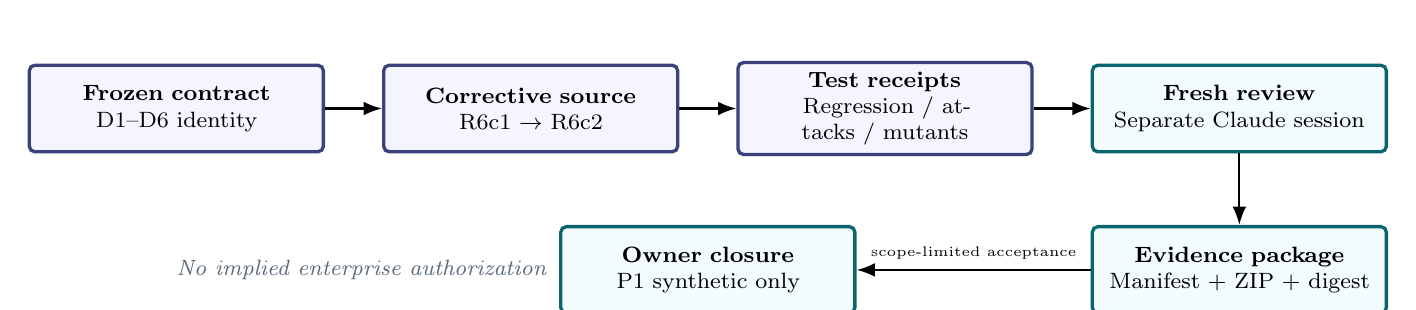
\begin{tikzpicture}[>=Latex,font=\footnotesize,
 b/.style={draw=royal,rounded corners=2pt,very thick,minimum height=11mm,text width=35mm,align=center,fill=blue!4},
 d/.style={draw=teal,rounded corners=2pt,very thick,minimum height=11mm,text width=35mm,align=center,fill=cyan!5}]
\node[b] (contract) at (0,0) {\textbf{Frozen contract}\\D1--D6 identity};
\node[b] (source) at (4.5,0) {\textbf{Corrective source}\\R6c1 $\to$ R6c2};
\node[b] (test) at (9,0) {\textbf{Test receipts}\\Regression / attacks / mutants};
\node[d] (review) at (13.5,0) {\textbf{Fresh review}\\Separate Claude session};
\node[d] (bundle) at (13.5,-2.05) {\textbf{Evidence package}\\Manifest + ZIP + digest};
\node[d] (owner) at (6.75,-2.05) {\textbf{Owner closure}\\P1 synthetic only};
\draw[->,thick] (contract)--(source);
\draw[->,thick] (source)--(test);
\draw[->,thick] (test)--(review);
\draw[->,thick] (review)--(bundle);
\draw[->,thick] (bundle)-- node[above,font=\tiny]{scope-limited acceptance}(owner);
\node[font=\footnotesize\itshape,color=muted] at (2.35,-2.05) {No implied enterprise authorization};
\end{tikzpicture}
\caption{Claim-to-evidence ladder for R6. The owner-local read-only audit verified archive and receipt bytes; the manuscript preparation environment did not rerun tests or directly access the private package.}
\label{fig:ladder}
\end{figure*}

\section{Reproducibility and Evidence Discipline}
\subsection{Three levels of reproducibility}
\textbf{Artifact identity.} Recheck exact frozen schema bytes, MCR3 Git commit/tree identities, stage-specific manifest hashes, and R6 archive bytes. \textbf{Offline deterministic reproduction.} Re-execute canonical qualification, synthetic scenarios, reviewer-authored regressions, mutation probes and manifest verification on a separately provisioned machine. \textbf{Enterprise reproduction.} Independently obtain and exercise approved real identity, policy, adapter, SAP or other enterprise-system readback against target-side predicates. The reported R6 tests and subsequent owner-local archive audit support bounded artifact identity and receipt claims. The executor performed offline tests; this paper neither independently reruns them nor claims enterprise reproduction.

\subsection{Provenance chain and exact anchors}
The MCR 3.0 merged reference commit is \texttt{7326207ed86b\allowbreak 258ffa233e37\allowbreak a1e4f611a816\allowbreak aa55}; its expected tree is \texttt{30b98ce0921d\allowbreak 706c75c3da0b\allowbreak 274378bec224\allowbreak fc6a}. Because the historical main checkout lacked the required local Git object, R5A recovered it in an isolated proof repository rather than resetting the working checkout. This is a meaningful scientific control: a commit string in a report is weaker than verification of the actual object and tree. The frozen R5 Class A archive digest is \texttt{1fcf28270f8c\allowbreak fd403f634214\allowbreak cc916cb4b08f\allowbreak 6a0a392f8be1\allowbreak 7cc8ecb76a61\allowbreak 2bb7}. Full D1--D6 digests appear in Table~\ref{tab:contracts}. The R6 package hash is recorded above. None of these hex strings has been newly computed in this environment.

\subsection{Reproduction protocol}
A responsible independent reviewer should: (i) obtain the owner-authorized R6 archive directly, (ii) verify its SHA-256 against the recorded value, (iii) validate the manifest and freeze-specific schema hashes, (iv) recover and inspect the exact MCR3 Git tree without changing historical workspaces, (v) re-run the R6c2 canonical suite, (vi) separately run the unchanged historical suite, (vii) inspect the reconciliation policy and supplementary mutation probes, (viii) check that the independent-review artifacts are attributable to a fresh session, and (ix) issue a classification that preserves every failure or uncertainty rather than editing past receipts. The current manuscript supplies a method and anchors, not that execution.

\subsection{Claim-to-evidence register}
\begin{table}[t]
\centering\caption{Evidence confidence and boundaries used throughout.}
\label{tab:claim}
\footnotesize
\begin{tabularx}{\columnwidth}{@{}p{0.42\columnwidth}X@{}}
\toprule
\textbf{Claim class} & \textbf{Paper treatment}\\\midrule
Frozen contracts / hashes & Reported in R7 handover + owner closure record\\
R6 numeric test results & Codex-supplied final receipt text; not rerun here\\
Fresh Claude verdict & Session ID and PASS disclosed; reviewer log not re-audited here\\
Owner closure authority & Explicit October 26 owner message; not a cryptographic signature\\
Architecture / equations & Authorial design abstractions; not observed API behavior\\
Class B / SAP / production & Not assessed; no corresponding PASS claim\\\bottomrule
\end{tabularx}
\end{table}

\subsection{Data and artifact availability}
The full R6 evidence ZIP and execution receipt were reported at private Windows paths under \code{[owner-held private R6 evidence directory]}. The PDF you are reading is a manuscript artifact created from supplied textual engineering records; it is not a publication of that entire evidence package. No publicly downloadable MCR 4.0 reproducibility release, Zenodo record, DOI, public peer review, or production deployment is established here. The existence of an MCR repository does not establish publication permission for the R6 package.

\section{Discussion and Design Implications}
\subsection{Agent capability is a controlled transition}
The main architectural claim is that capability discovery is insufficient. The runtime must ask which target is selected, who authorizes the operation, how long that approval remains valid, what attempts are permitted, what constitutes safe recovery, and which independent observations demonstrate the result. This separates an attractive conversational agent from an auditable engineering system. It also separates \emph{product usefulness} from \emph{proof of permitted action}.

\subsection{A boundary between assurance and orchestration}
ACLA, EAF and MCR should not collapse into one opaque component. Context is a data selection and provenance problem; assurance is an authority and outcome-assessment problem; execution is a capability binding, state, retry, and evidence sequencing problem. The interfaces must be interoperable without granting adjacent systems unauthorized decision rights. The approved Class A contracts express the beginnings of this division, but integration is deliberately left for later authorization.

\subsection{What the negative results teach}
The R4B review contradicted an early green test story by finding weaknesses in authority expiry, nonce/call-budget enforcement, unknown-state recovery and observer integrity. R5 introduced further hardening but exposed a reproducibility dependency on an unavailable frozen Git object. R5A repaired that provenance issue without resetting unrelated source and preserved an awkward but legitimate raw-runner failure. R6 finally adopted a reconciled qualification method with supplementary mutation probes and fresh review. The trajectory demonstrates why a scientific engineering program should retain failures and rejected assumptions, rather than produce a rewritten history in which every release was always correct.

\subsection{System-of-record authority remains external}
Even a perfectly deterministic orchestrator cannot manufacture SAP activation, enterprise policy truth, or transactional readback. Real operations need current identity and authorization issuers, target metadata, environment-specific controls, independent observation rights, and business-level predicates. Those requirements are not solved by synthetic tests or by hashes. A future MCR program should therefore preserve one-way, explicitly authorized promotion from Class A research to any Class B evaluation and then to separately approved live environments.

\section{Future Work and Release Gates}
Future studies may test real Class B adapters, policy-authority freshness under clock skew, durable recovery under network partition and ambiguous remote commit, external observer compromise, contract evolution under migration, controlled multi-provider missions, latency and cost per verified outcome, and independent reproducibility by non-participating reviewers. Such work must be planned separately: no Class B engineering, enterprise credentials, SAP writes, production changes, or Git publication is authorized by the P1 closure. Table~\ref{tab:future} states the approval threshold without implying that the steps have been undertaken.

\begin{table}[t]
\centering\caption{Next-phase decision gates (proposed; not authorized).}
\label{tab:future}
\footnotesize
\begin{tabularx}{\columnwidth}{@{}p{0.3\columnwidth}X@{}}
\toprule
\textbf{Gate} & \textbf{Required proof or decision}\\\midrule
G0 Scope & Owner-approved mission, targets and permitted operations\\
G1 Adapters & Versioned Class B schemas; adversarial interface review\\
G2 Authority & Live issuer/expiry/revocation readback\\
G3 Observation & Target-side readback with independent predicates\\
G4 Recovery & Ambiguous-commit and idempotency behavior\\
G5 Reproducibility & Independent rerun; signed evidence where policy requires\\
G6 Release & Human production approval; operations/rollback proof\\\bottomrule
\end{tabularx}
\end{table}

\section{Responsible Research and AI Assistance}
The author directed the MCR research program, approved the frozen Class A contract digests, received engineering reviews, and explicitly authorized the bounded P1 closure decision. Codex acted as primary engineering executor for the reported R6 qualification. Fresh Claude Code sessions acted as technical adversarial reviewers, including a third fresh R6 review. Generative AI also assisted this manuscript's structure, source comparison, reference discovery, and editorial assembly. The author remains responsible for the final claims, disclosures, verification of any third-party or private evidence, and publication decisions. AI-generated review is not represented as peer review, human certification, or cryptographic attestation. The paper includes no private enterprise credentials, no SAP write procedure, and no claim that such operations occurred.

The owner-approved closure is \code{MCR\_\allowbreak R4\_\allowbreak 0\_\allowbreak P1\_\allowbreak CLOSED\_\allowbreak BOUNDED\_\allowbreak SYNTHETIC\_\allowbreak RESEARCH}. It does not authorize public release of private research artifacts. Reviewer-reported evidence-field limitations and an incidental \code{\string~/.gnupg} side effect remain disclosed in the owner closure record, not asserted to have been independently remediated.

\section{Conclusion}
MCR 4.0 addresses a common failure of agentic system descriptions: confusing intent, permission, action and observed outcome. The research proposes a deterministic execution-and-evidence boundary that sits alongside context compilation and independent assurance, without inheriting authority from either. A frozen six-contract Class A baseline and an extended synthetic adversarial program exposed important faults, drove isolated corrections, preserved conflicting historical tests, and culminated in an executor-reported final R6 qualification with an independently executed fresh Claude review. The owner closed Phase 1 as bounded synthetic research on October 26, 2026.

The conclusion is deliberately constrained. These results support a research-level account of how to \emph{design and test} safe mission transitions; they do not establish live enterprise interoperability, SAP business outcomes, production safety, or superiority over alternate agent architectures. The enduring systems principle is straightforward: \emph{an agent's ability to act is not the same as its authority to act, and a report of completion is not proof of outcome.}

\section*{Data, Artifact, and Ownership Statement}
The research family uses the named author and independent-research affiliation shown above. The author retains responsibility for interpretation and release permissions. This manuscript is an author-facing publication draft backed by the supplied MCR 4.0 handover and closure record; it contains no newly executed R6 results. The private R6 evidence artifact is withheld; an owner-local read-only auditor subsequently reported verification of archive bytes and receipts, while the manuscript preparation environment did not independently access or rerun the private artifact. No Zenodo DOI or public release URL has been invented. Final public publication, licensing, sanitization and immutable artifact deposition require separate owner approval.

\section*{Acknowledgments}
The author acknowledges AI-assisted engineering and adversarial review through Codex and Claude Code, and recognizes the distinction between tool-assisted review, owner acceptance and formal external scientific peer review. The operational evidence remains bounded by the original verification and governance contracts.

\begin{thebibliography}{99}\setlength{\itemsep}{1pt}\footnotesize
\bibitem{deshpandeACLA} P. Deshpande, ``From Persistent Memory to Mission Working Sets: An Authority-Aware Context Lifecycle Architecture for Agentic AI,'' version 1.1.0, final post-review manuscript, 2026. Referenced author research paper; no claim that its findings are MCR measurements.
\bibitem{deshpandeEAF} P. Deshpande, ``Enterprise Agent Framework (EAF): Minimum Authoritative Working Sets and Closed-Loop Outcome Assurance for Enterprise AI Agents,'' public research artifact v1.1.0, 2026. Zenodo DOI:10.5281/zenodo.22193673. Original EAF research, not MCR 4.0 integrated runtime evidence.
\bibitem{nistAirmf} E. Tabassi, ``Artificial Intelligence Risk Management Framework (AI RMF 1.0),'' NIST AI 100-1, 2023. doi:10.6028/NIST.AI.100-1.
\bibitem{nistGai} C. Autio \emph{et al.}, ``Artificial Intelligence Risk Management Framework: Generative Artificial Intelligence Profile,'' NIST AI 600-1, 2024. doi:10.6028/NIST.AI.600-1.
\bibitem{nist80053} Joint Task Force, ``Security and Privacy Controls for Information Systems and Organizations,'' NIST SP 800-53 Rev. 5, 2020. doi:10.6028/NIST.SP.800-53r5.
\bibitem{owaspAgency} OWASP GenAI Security Project, ``LLM06:2025 Excessive Agency,'' OWASP Top 10 for LLM Applications (2025 reference classification), \url{https://genai.owasp.org/llmrisk/llm062025-excessive-agency/}, accessed 2026-10-26.
\bibitem{lamport1978} L. Lamport, ``Time, Clocks, and the Ordering of Events in a Distributed System,'' \emph{Communications of the ACM}, vol. 21, no. 7, pp. 558--565, 1978. doi:10.1145/359545.359563.
\bibitem{rfc8785} A. Rundgren, B. Jordan, and S. Erdtman, ``JSON Canonicalization Scheme (JCS),'' RFC 8785, 2020. doi:10.17487/RFC8785.
\bibitem{intoto2019} S. Torres-Arias \emph{et al.}, ``in-toto: Providing farm-to-table guarantees for bits and bytes,'' \emph{28th USENIX Security Symposium}, pp. 1393--1410, 2019.
\bibitem{slsa11} Open Source Security Foundation / SLSA contributors, ``SLSA Specification v1.1,'' \url{https://slsa.dev/spec/v1.1/}, accessed 2026-10-26.
\bibitem{jia2011} Y. Jia and M. Harman, ``An Analysis and Survey of the Development of Mutation Testing,'' \emph{IEEE Transactions on Software Engineering}, vol. 37, no. 5, pp. 649--678, 2011. doi:10.1109/TSE.2010.62.
\bibitem{mcrHandover} P. Deshpande (research owner), ``MCR 4.0---Engineering Handover to Next Chat,'' \code{MCR\_\allowbreak R4\_\allowbreak 0\_\allowbreak P1\_\allowbreak E2E\_\allowbreak ENGINEERING\_\allowbreak HANDOVER\_\allowbreak R7}, internal engineering record, 26 Oct. 2026. Text supplied for manuscript preparation.
\bibitem{mcrClosure} P. Deshpande (research owner), ``MCR 4.0 P1---Owner Closure Record R1,'' \code{MCR\_\allowbreak R4\_\allowbreak 0\_\allowbreak P1\_\allowbreak OWNER\_\allowbreak CLOSURE\_\allowbreak R1}, internal scope-limited decision record, 26 Oct. 2026.
\bibitem{mcrR6} Codex (primary engineering executor), ``MCR R4.0 P1 End-to-End Ownership, Independent Qualification and Closure R6,'' final execution receipt summarized in owner-supplied conversation, 26 Oct. 2026. Original JSON/ZIP private; subsequent owner-local read-only audit reported archival integrity without a new execution run.
\bibitem{mcrAudit} P. Deshpande (research owner), ``MCR R6 Evidence Audit,'' owner-supplied read-only audit receipt, 26 Oct. 2026. Reports 30,869/30,869 manifest hash/size checks, retains raw historical exceptions, and classifies the private archive as not suitable for direct public release. Original report reviewed as text; private evidence bytes not examined by this manuscript preparation environment.
\end{thebibliography}

\appendix
\small
\section{Exact Baseline and Packaging Identifiers}
\noindent\textbf{MCR 3.0 reference.} Qualified merged main: \texttt{7326207ed86b\allowbreak 258ffa233e37\allowbreak a1e4f611a816\allowbreak aa55}. Expected tree: \texttt{30b98ce0921d\allowbreak 706c75c3da0b\allowbreak 274378bec224\allowbreak fc6a}. Frozen recovered Git proof: \code{[owner-held private frozen Git proof directory]}.\par
\noindent\textbf{MCR 4.0 Class A.} Baseline version 1.0.0, state \code{FROZEN\_\allowbreak OWNER\_\allowbreak APPROVED\_\allowbreak CLASS\_\allowbreak A}, owner-approved D1--D6 exact digests in Table~\ref{tab:contracts}. R5 archive digest: \texttt{1fcf28270f8c\allowbreak fd403f634214\allowbreak cc916cb4b08f\allowbreak 6a0a392f8be1\allowbreak 7cc8ecb76a61\allowbreak 2bb7}.\par
\noindent\textbf{R6 evidence.} \code{R6\_\allowbreak EVIDENCE\_\allowbreak PACKAGE.zip}; \code{14\_\allowbreak FINAL\_\allowbreak EXECUTION\_\allowbreak RECEIPT.json}; reported ZIP SHA-256: \texttt{cf3f7162d090\allowbreak 70ca86840e74\allowbreak 1f3e81a1baa5\allowbreak ff9350d4dd1a\allowbreak 8eac156f7250\allowbreak 074c}. Local archive location: \code{[owner-held private R6 evidence directory]}. The owner-local auditor reported checking 30,869/30,869 manifest entries; this manuscript environment did not itself open their private bytes.

\section{Historical Defect Register}
\noindent\textbf{F1.} Invalid or incorrectly compared authority expiry. \textbf{F2.} Missing envelope digest, maxCalls and nonce controls. \textbf{F3.} UNKNOWN resume improperly representing prior ALLOW as current. \textbf{F4.} Observer provenance and source-trust weakness. \textbf{F5.} Non-committed scenario counters/observations. \textbf{F6.} Observer exception can wedge idempotency key. \textbf{F7.} Frozen MCR3 Git object not locally verified. \textbf{F8.} Untracked generated \code{\_\allowbreak \_\allowbreak pycache\_\allowbreak \_\allowbreak } artifacts. The R6 supplied receipt states bounded correction and independent qualification; this paper does not provide source-level proof of each fix.

\section{Reconciliation and Decision Vocabulary}
\noindent\textbf{Raw historical result:} unmodified reviewer suite 38/40 and raw harness exit 1. \textbf{Reconciled current result:} 40/40 current reviewer checks and R6c2 canonical runner 26/26 with exit 0. \textbf{Owner closure:} \code{MCR\_\allowbreak R4\_\allowbreak 0\_\allowbreak P1\_\allowbreak CLOSED\_\allowbreak BOUNDED\_\allowbreak SYNTHETIC\_\allowbreak RESEARCH}. \textbf{Enterprise status:} \code{MCR\_\allowbreak R4\_\allowbreak 0\_\allowbreak ENTERPRISE\_\allowbreak QUALIFICATION\_\allowbreak NOT\_\allowbreak AUTHORIZED}. The reviewer-test adoption decision remains separately pending. Both narratives must survive any subsequent manuscript or artifact migration.

\section{Proposed Independent Replication Checklist}
\begin{enumerate}
\item Obtain the exact package by an owner-approved channel and verify the recorded ZIP SHA-256.
\item Verify manifest count and all file hashes, then inspect D1--D6 contract digests against exact archived bytes.
\item Recover the MCR3 Git object and tree in an isolated read-only checkout; avoid mutation of the primary workspace.
\item Execute R6c2 canonical runner and record command, environment, outputs, exit code and complete receipt.
\item Execute retained historical raw reviewer tests \emph{without changing expected outcomes}; preserve their original 38/40 result.
\item Examine the reconciliation policy, two superseded assertions and new mandatory checks for soundness.
\item Replay the adversarial reviewer tests and all 45 distinct mutation cases, distinguishing raw kills, supplementary kills and redundancy decisions.
\item Verify independent-review attribution and assess whether any reviewer evidence fields are excluded from commitments.
\item Inspect incidental side effects such as the reported GnuPG directory creation; confirm no secret leakage, without assuming remediation.
\item Produce an independent written PASS/HOLD decision, with no live-system or production implications absent new approval.
\end{enumerate}

\balance
\end{document}
